

\begin{figure}[H]
    \centering
    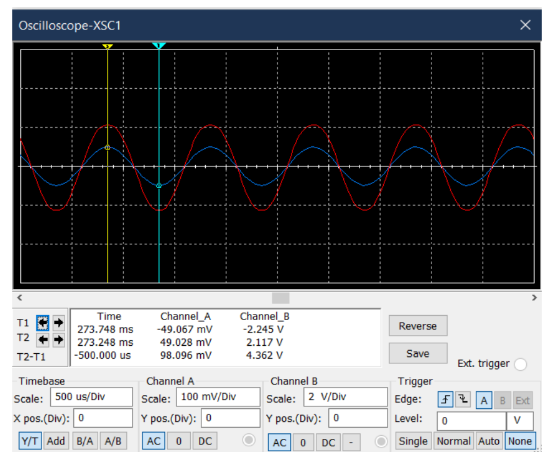
\includegraphics[width=16cm]{Pictures/Waveform-RL.png}
    \caption{{The waveform of input voltage and output voltage for $R_L = 1k\ohm$}}
    \label{waveform-rl-dia}
\end{figure}

\begin{table}[H]
\centering
\begin{tabular}{|c|c|c|}
\hline\hline
\textbf{\(V_{I, P-P}\) [mV]} & \textbf{\(V_{O, P-P}\) [V]} & \textbf{\(A_{vo}\) [V/V]} \\ \hline
98.096 & 4.362 & 44.467 \\ \hline\hline
\end{tabular}
\caption{\(V_I\), \(V_O\), and \(A_{vo}\) (Loaded Voltage Gain) for \(R_L = 1 \, k\Omega\), \(f = 1 \, kHz\)}
\label{table:E1}
\end{table}


\begin{figure}[H]
    \centering
    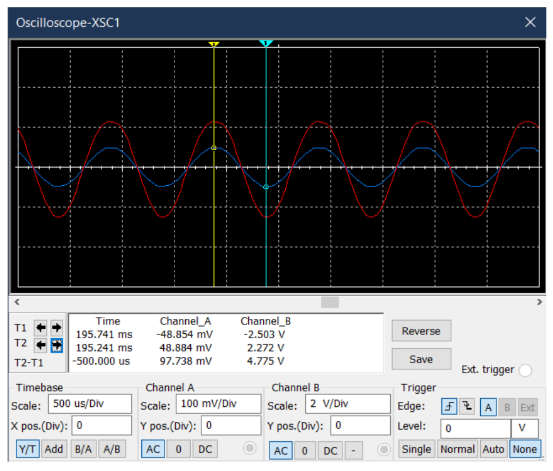
\includegraphics[width=16cm]{Pictures/Waveform.png}
    \caption{{The waveform of input voltage and output voltage for $R_L = \infty$}}
    \label{waveform-dia}
\end{figure}


\begin{table}[H]
\centering
\begin{tabular}{|c|c|c|}
\hline
\textbf{\(V_{I, P-P}\) [mV]} & \textbf{\(V_{O, P-P}\) [V]} & \textbf{\(A_{vo}\) [V/V]} \\ \hline
97.738 & 4.775 & 48.855 \\ \hline
\end{tabular}
\caption{\(V_I\), \(V_O\), and \(A_{vo}\) (No Load Voltage Gain) for \(R_L = \infty\), \(f = 1 \, kHz\)}
\label{table:E2}
\end{table}

\begin{figure}[H]
    \centering
    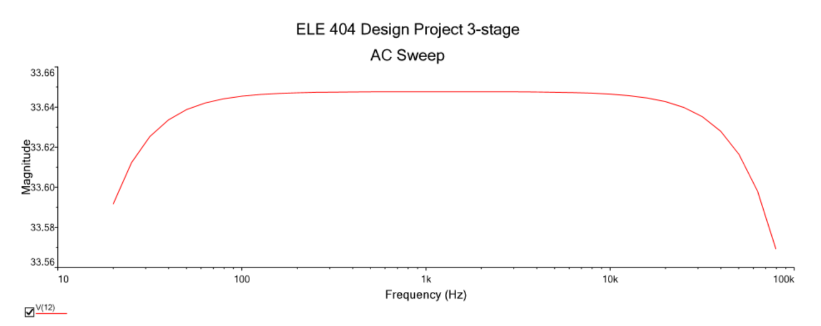
\includegraphics[width=16cm]{Pictures/Frequency-Response.png}
    \caption{{Frequency Response}}
    \label{freq-response}
\end{figure}
